In this section we will provide the methods of solar cell characterisation and the quantities which are connected to it. More information can be read in \ref{pv}

\subsection{Properties of sunlight}

The most important characteristics of the solar light are described by radiometric quantities. We will just state few of them. To finely describe the effects of sunlight we need to know:

\begin{itemize}
\item Spectrum of the incident light
\item Radiation angle
\item Radiant power density
\end{itemize}

\subsubsection{Photon flux}
$\Phi$ is simply stated as the number of photons per unit area in a fraction of time. We can then define the photon flux density to further divide it on the incident light wavelength. When we multiply $\phi _{\lambda } $ by the photon energy we get the energy per unit time, which is simply the power density. 

\begin{equation}
\frac{\partial ^2 P_\lambda }{\partial ^2 x^2} = \phi _ {\lambda } \frac{hc}{\lambda }
\end{equation}

\subsubsection{Spectral Irradiance}

It is most common quantity to describe a light source. It is the power density for a certain photon frequency. 

\begin{equation}
I_{e,\lambda } = \frac{\partial ^2 P_\lambda }{\partial ^2 x^2} = \phi_\lambda \cdot \frac{hc}{\lambda }
\end{equation}

\subsubsection{Blackbody radiation}

Derived by Planck, this radiation law is described with spectral irradiance\cite{planck}:

\begin{equation}
I_\lambda = \frac{2\pi hc^2}{\lambda^5(e^{\frac{hc}{k\lambda T}}-1)}
\end{equation}

\subsection{Solar Cell Operation}

For a solar cell to generate current, the following main processes must be present. First one is the possibility to absorb photons from incident light so we can generate carriers. We must remember that minority carriers are only stable for a minority carrier lifetime before recombination. Therefore, before this time, we need to collect those carriers to spatially disallow carriers to recombine. Ideally, if we create pair in the n region, the electric field sweeps the minority carrier through the junction to the place where it becomes majority carrier. In a short circuit scenario, two carriers ideally meet together after flowing through the external circuit. 

The fact that the carriers must "live" through the distance needed to separate them is described by collection probability, which depends on the diffusion length and surface properties. 

The number of carriers collected in the solar cell compared to the number of incident photons describes the more macroscopic ability of the device. It is called a \textbf{quantum efficiency} 

\begin{equation}
Q.E=\frac{number  of  carriers  collected}{number  of  incident  photons}
\end{equation}
It is strictly dependent also on the absorption, so directly on the wavelength of incident photons. 

\begin{figure}
\centering
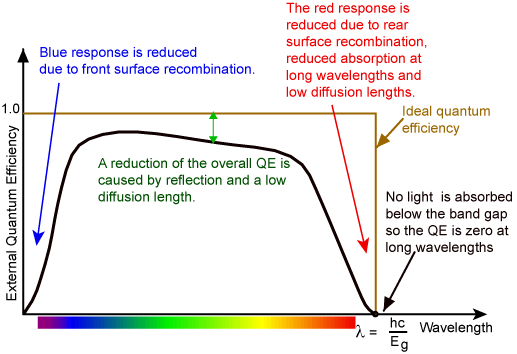
\includegraphics[width =0.6\textwidth]{ch2/QE}
\caption{Quantum efficiency of an ideal silicon solar cell \cite{pv}}
\end{figure}

It is also possible to describe an external QE(EQE), which also includes some optical effect such as reflection. 

\subsection{Solar Cell Parameters}
Here, we will state the most important parameters for solar cell characterisation, we will simply tell what do they stand for and how to measure them. 

\subsubsection{Short-Circuit Current}
$I_{sc}$ is the current that flows through the device providing that the voltage is zero across it(especially when we have short circuit). It comes directly from the generated carriers due to photogeneration and is connected to how well the structure can collect them or how strong the recombination processes are. It depends on:

\begin{itemize}
\item incident photons number(linear dependence on the incident power)
\item solar cell area
\item light spectrum
\item optical losses(f.e. absorption, reflection etc.)
\item real collection efficiency(its' probability)
\end{itemize}

We can clearly see, that this parameter allows us to differentiate between solar cells when comparing the ability to store generated carriers.(Remember, short-circuit current is not always the light generated current due to possible high series resistance).

\subsubsection{Open-Circuit Voltage}

$V_{oc}$ is the voltage that is maximally available when using the solar cell. For that voltage, the current through the circuit needs to be zero. It states the forward bias that we need to put to compensate the light generated current. $V_{oc}$ is logarithmically dependent on the incident photon power and it decreases linearly with temperature. 

\subsubsection{Fill Factor}

When speaking about the above short-circuit current and open circuit voltage we are meaning the maximal current and voltage that we can achieve in the solar cell. Of course, as the momentary power is just their multiplication, therefore, at those times when we get each of the two listed quantities, the power is equal to zero. In order to still describe maximal power of the solar cell, people tend to use the \textbf{fill factor} FF.

\begin{equation}
FF = \frac{P_{max}}{V_{oc}I_{sc}}
\end{equation}

where $P_{max}$ is the maximal power achieved by the solar cell. It is the   embodiment of the "squareness" of a solar cell. The higher the open circuit voltage, the bigger the FF. 

\subsubsection{PCE}

From the FF we can derive another, probably most useful quantity, which has been yet used in the former chapters. This quantity is the \textbf{power conversion efficiency} PCE. It is a ratio of energy from the solar cell to the summary energy income from the Sun. 

\begin{equation}
\eta = \frac{V_{oc}I_{sc}FF}{P_{in}}
\end{equation}

where $\eta$ is the PCE and $P_{in}$ is the sunlight power. 

\subsection{Shockley-Queisser limit}

Also known as a detailed balance. It was a derivation of an idealistic maximum efficiency of a solar cell based on a p-n junction made by Shockley and Queisser in 1961\cite{limit}. The most common form of the implementation comes with fundamental assumptions:

\begin{itemize}
\item We have finite mobility, so the collection of the carriers can be performed anywhere.
\item For wavelengths exceeding the band gap we have a complete absorption of photons.
\end{itemize}


In the principle, only photons with energy greater than the band gap can be absorbed and used in the generation of electron hole pairs. Generally, the electrons occupy the lowest level of the conduction band and so the exceed energy is released in heat in thermalisation process. For the idealistic model, they assumed that each photon with sufficient energy generates electronic charge q at voltage $V_g=hv_g/e$. $E_g$ is the threshold for energy as the band gap, and as we stated before, we assume that all photons are absorbed above, so the function a(E) is equal to zero below $E_g$ and unity otherwise. We can say that from the generated charge, the photocurrent density when shined with the photon flux $\Phi _{sun}$ is:

\begin{equation}
J_{sc} = q \int_0 ^{\infty } \Phi _{sun}(E)a(E)dE=q \int_{E_g} ^{\infty } \Phi _{sun}(E)dE
\end{equation}

Of course, to conceive the thermodynamic equilibrium, there needs to be an opposite process to absorption. We assume that the light emitted from the Sun is in the form of Blackbody radiation, as is the solar cell. The amount of radiation absorbed is the same as the emitted from the device to the environment with the same temperature. Therefore further it involves using a Planck Blackbody generalized formula for different energies above the band gap. Non-equilibrium radiation is only in a situation where the non-zero chemical potential of a radiation is present, and that is basically equal to a Quasi-Fermi level splitting(we have stated before that the splitting of a Fermi level is a non-equilibrium process). The photon flux emitted by a Blackbody with a bias voltage V is equal:

\begin{equation}
\phi (V,E) = \frac{2\pi E^2}{h^3c^2}\frac{a(E)}{e^{(( E-qV)/kT) - 1}}
\end{equation}

with c as the light vacuum velocity, k as a Boltzman constant, T as a temperature. This emission is connected with a recombination current density $J_r = q\Phi _e$, where $\Phi  _e$ is an integration of the flux density over all energies. In thermal equilibrium both currents are equal. When we apply voltage, we know that the current is a Shockley equation (Eq. \ref{eq:Shockley}. Maximal voltage is ideally the $V_{oc} = kT/qln(J_{sc}/J_{0} + 1)$, yes, it is the open-circuit voltage and $J_0 = q \int a(E)\phi _{abs}(E) dE$. Now, connecting this with AM1.5G spectrum Fig.(\ref{fig:AM15}), which is a standard spectrum for using solar cells, we can get that normally, for solar cells with band gap within 1eV to 1.5eV, we can get the maximal efficiency of 33\%  . \cite{limit}

\begin{figure}
\centering
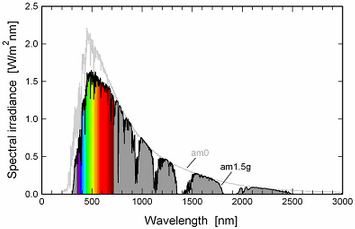
\includegraphics[width = 0.85\textwidth]{ch2/am15}
\caption{AM1.5 irradiation at Earth surface\ref{am} and AM0 at Earth's orbit}
\label{AM15}
\end{figure}

In exceeding the SQ limit we can use for example:
\begin{itemize}
\item Tandems
\item Magneto-optic devices
\item Hot carriers(strong electric field effects)
\item Multiple exciton generation(as in Quantum Dot Solar Cells it is possible to create more than one exciton from one photon!)
\end{itemize}

\subsection{Effective resistance}

To include some of the resistive effect on the solar cell and still use a model similar to the idealistic one, one uses series resistance and shunt resistance. Their main impact is on the FF of the device. Their dependence is on the geometrical properties of the solar cell. 

The series resistance has it's origin at three physical places: the emitter-base current, contact metal-semiconductor and top/rare contacts resistances. To include it we simply write the current equation as. 

\begin{equation}
I=I_{lg} - I_0e^{\frac{q(V+IR_s)}{nkT}}
\end{equation}

where n is an ideality factor and $R_s$ is the series resistance. The rest is taken from Eq.(\ref{eq:Shockley}).

For the shunt resistance the case is about the defects from the manufacturing. It simply takes away the factor $\frac{V+IR_s}{R_{sh}}$, where $R_{sh}$ is the shunt resistance. \cite{pv}